% Created 2018-12-27 Thu 19:58
% Intended LaTeX compiler: pdflatex
\documentclass[12pt, notitlepage, onecolumn, amsmath, amssymb, aps]{revtex4-1}

\usepackage[utf8]{inputenc}
\usepackage[T1]{fontenc}
\usepackage{graphicx}
\usepackage{grffile}
\usepackage{wrapfig}
\usepackage{rotating}
\usepackage[normalem]{ulem}
\usepackage{amsmath}
\usepackage{textcomp}
\usepackage{amssymb}
\usepackage{capt-of}
\usepackage{color}
\usepackage{hyperref}
\usepackage{dcolumn}
\usepackage{bm}
\usepackage{natbib}
\usepackage{float}
\usepackage{subcaption}

% \bibliographystyle{abbrvnat}
\bibliographystyle{unsrtnat}
%\date{\today}
\title{}
\hypersetup{
 pdfauthor={Yilun Guan},
 pdftitle={},
 pdfkeywords={},
 pdfsubject={},
 pdfcreator={Emacs 25.2.2 (Org mode 9.1.11)}, 
 pdflang={English}}
\begin{document}

%================== Begin of Header ========================
%\preprint{APS/123-QED}
\title{Research Summary}
\author{Hongbo Cai \\{\small Supervisor: Arthur Kosowsky}}
\affiliation{Department of Physics and Astronomy, University of Pittsburgh}
%\date{\today}
%\pacs{Valid PACS appear here}
%\keywords{Suggested keywords}
\maketitle
% ================== End of Header =========================
\newcommand{\edit}[1]{\textcolor{red}{(#1)}}
\vspace{-1.5cm}
\section{Introduction to Cosmic Microwave Background(CMB)}
\label{sec:org8852578}

Anisotropies in the cosmic mircrowave background(CMB) radiation have provided a weath of information about cosmological model that describes the contents and evolution of the universe\cite{Staggs:2018gvf}. We extract multipoles from CMB temperature anisotropies(T) and polarization anisotropies(E,B) which traces the behaviour at 400 000 years of cosmic time, as well as from the signals imprinted at later times due to scattering from galaxy clusters, from the motion of electrons ionized, and from gravitationl lensing. FIG 1. shows the full sky temperature anisotropies from Planck experiment(Satillite-based).
\begin{figure}[h]
\includegraphics[width=0.8\textwidth]{planck.jpg}
\caption{The 2018 Planck map of the temeprature anisotropies of the CMB}
\end{figure}
Ground-based experiments such as Advanced Atacama Cosmology Telescope(AdvACT)\cite{Henderson:2015nzj} and upcoming the Simons Observatory\cite{Ade:2018sbj} can have much better resolution. I am now a member of the both collaborations.

\section{CMB Lensing reconstruction on the curved sky}
\label{sec:org8852578}


Cosmic Microwave Background(CMB) photons are gravitationlly lensed by the large scale mass distribution. This effect is called CMB lensing. CMB temperature anisotropies(T) and polarization anisotropies(E,B) are distorted by CMB lensing. We can use deflection field or lensing potential to discribe CMB lensing\cite{Lewis:2006fu}. It is expected to amongst the most powerful cosmological tools for ongoing and upcoming CMB experiments which will help find out premordial gravitationl waves, constrain cosmological parameters, constrain neutrino mass and understand the properties of dark energy and . So it is important to reconstruct the CMB lensing according to the oberved CMB temperature and polarization anisotropies. The process of reconstructing lensing potential is called CMB lensing reconstruction.

There are two aspects where we can see CMB lensing effects:
1.CMB lensing modulates CMB temperature and polarization power spectra(2 point power spectrum). Statistical anisotropy is induced.
2.CMB lensing produces higher-order correlations between the multipole moments. Off-diagonal mode-coupling between map harmonics can be seen. The off-diagonal mode coupling is proportional to lensing potential.\cite{Hu:2001kj}

\begin{equation}
  \left\langle a_{l}^{m} b_{l^{\prime}}^{m^{\prime}}\right\rangle= C_{l}^{a b} \delta_{l l^{\prime}} \delta_{m-m^{\prime}}(-1)^{m}
\end{equation}

\begin{equation}
  \left.\left\langle a_{l}^{m} b_{l^{\prime}}^{m^{\prime}}\right\rangle\right|_{\text {lens }}=C_{l}^{a b} \delta_{l l^{\prime}} \delta_{m-m^{\prime}}(-1)^{m}+\sum_{L M}(-1)^{M}\left(\begin{array}{ccc}
{l} & {l^{\prime}} & {L} \\
{m} & {m^{\prime}} & {-M}
\end{array}\right) f_{l L l^{\prime}}^{\alpha} \phi_{L}^{M}
\end{equation}
Eq(1) and Eq(2) are the covariance of unlensed and lensed CMB multipoles respectively. \(a_{l}^{m} \)and \(b_{l}^{m} \)  are multipoles for T, E or B-mode multipoles. \(\phi_{l}^{m}\) is lensing potential multipole. As we can see, the multipole covariance gained an extra term which is proportional to lensing potential and Wigner-3j symbols. 

For primordial gravitationl waves, CMB lensing can be an important source of confusion\cite{Lewis:2006fu}. Density perturbations in the linear regime generate only the so-called E-mode polarization\cite{Kamionkowski:1996ks}. Lensing converts E-mode polarization to B-mode polarization.\cite{Zaldarriaga:1998ar}. Gravitationl waves can also produce B-mode polarization\cite{Hu:2000ee}. Removing the lensing-generated B-mode is called delensing.

To obtain lensing potential, we can take quadratic combinations of CMB fields and construct quadratic estimators with minimum variance\cite{Hu:2000ee}. On small angular scales \(L>10^2\), we are able to neglect the curvature of the sky and apply flat sky estimators\cite{Hu:2001kj}. Since lensing is most sensitive to the projected potential at \(L<10^2\) or several degrees on the sky, we need consider the curvature of the sky. In this study, we apply estimators for lensing potential on the curved sky provided by Ref\cite{Okamoto:2003zw} as shown is Eq(3):
\begin{equation}
  d_{L}^{\alpha M}=\frac{A_{L}^{\alpha}}{\sqrt{L(L+1)}} \sum_{l_{1} m_{1}} \sum_{l_{2} m_{2}}(-1)^{M}\left(\begin{array}{ccc}
{l_{1}} & {l_{2}} & {L} \\
{m_{1}} & {m_{2}} & {-M}
\end{array}\right) g_{l_{1} l_{2}}^{\alpha}(L) a_{l_{1}}^{m_{1}} b_{l_{2}}^{m_{2}}
\end{equation}


We reconstruct lensing potential and get noise properties for the full sky. This work is meant for improving the existing lensing reconstruction pipline in Advanced Atacama Cosmology Telescope(AdvACT) and Simons Obervatory(SO). This work now only works for the full sky using TT and EB estimators. And its performance is still limited by now as shown in FIG 2,  expected to be improved.

\begin{figure}[h]
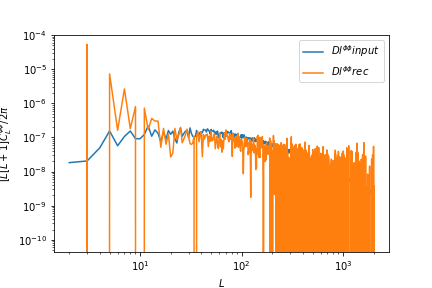
\includegraphics[width=0.8\textwidth]{Dl_phiphi_rec.png}
\caption{Input Lensing Potential and Reconstrued Lensing Potential}
\end{figure}

I've learned lensing reconstruction techniques from this work. These techniques are applied in the work shown in the section 2 below.



\section{Bias to CMB Lensing Reconstruction from Temperature Anisotropies due to Reionization kSZ}
\label{sec:org093d799}
In this work, we are investigating a bias to CMB lensing reconstruction from temperature anisotropies due to the reionization kSZ effect(kinematic Sunyaev-Zel'dovich effect) based on simulation.

There are several ongoing and upcoming experiments, including Advanced Atacama Cosmology Telescope(AdvACT)\cite{Henderson:2015nzj}, the South Pole Telescope-3G(SPT-3G)\cite{Benson:2014qhw}, the Simons Observatory\cite{Ade:2018sbj}, and CMB Stage-4(CMB-S4)\cite{Abazajian:2016yjj}. For these experiments, the CMB lensing power spectrum will be measured with signal-to-noise\((S/N)>100\). At this precision level, we are required to consider more about biases in CMB reconstruction. Most of the biases can be removed from primary CMB by a multifrequency component seperation methods, but they don't work for kSZ effect, since kSZ effect preserves blackbody spectrum of the CMB.\cite{Smith:2009pn}

kSZ effect is the Doppler shift of CMB photons induced by Compton-scattering off moving electrons(bulk velocity).\cite{Ferraro:2017fac}. The kSZ signal has its own intrinsic non-Gaussianity and its correlation with CMB lensing field is non-zero.\cite{Smith:2016lnt}.

This kSZ effect produces a CMB temperature change, \(\Theta^{\mathrm{kSZ}}(\hat{\mathbf{n}})=\Delta T^{\mathrm{kSZ}}(\hat{\mathbf{n}}) / T_{\mathrm{CMB}}\),
\begin{equation}
  \Theta^{\mathrm{kSZ}}(\hat{\mathbf{n}})=-\sigma \int \frac{d \eta}{1+z} e^{-\tau} n_{e}(\hat{\mathbf{n}}, \eta) \mathbf{v}_{e} \cdot \hat{\mathbf{n}}
\end{equation} \cite{Ferraro:2017fac},

where \(\sigma\) is the Compton scattering cross-section, \(\tau\) is the optical depth to Compton scattering, \(n_{e}\) is the physical free number density, \(mathbf{v}_{e}\) is the peculiar velocity of the electrons.
kSZ anisotropies can be produced when large fluctuation in electron density appears. There are two epochs when they can be produced: 1.a ``late-time'' contribution from redshifts \(0<z<6\) in which inhomogeneities are large due to gravitational growth of structure 2.earlier during the epoch of reionization(from first stars, \(6<z<20\)) when hydrogen gets ionized again by the ultraviolet radiation of the first structures and the fluctuations electron density are caused by the fluctuations in the ionization fraction.\cite{Ferraro:2017fac} \cite{Alvarez:2015xzu}. It is expected to be correlated with lensing field.

Simone Ferraro and J. Colin Hill  have investigated the case of ``late time'' kSZ in \cite{Ferraro:2017fac}. Accordin to their results, the bias induced by ``late time'' kSZ to CMB lensing auto-power spectrum measurements can be as large as approximately \(\%1\), \(\%6\), and \(\%8\) for Plank, CMB-S3, and CMB-S4, respectively, when using \(l_{max} = 4000\), and about half of that for \(l_{maxy} = 3000\). Thus, for CMB-S3 and CMB-S4 lensing measurements, the kSZ-induced bias cannot be neglected.

For the case of reionization kSZ, it could also contribute at some level. We are trying to estimate reionization-induced bias to CMB lensing reconstruction from temperature anisotropies based on lensed temperature anisotropies\cite{Stein:2020its} and reionization kSZ map from Ref\cite{Alvarez:2015xzu}. In this study, we apply flat-sky reconstruction pipeline to cutout patchy lensed temperature maps with reionization kSZ and without reionization kSZ given different noise levels, beam sizes and \(l_{max}\). We compare their reconstruction lensing convergence powerspectra and see how much bias the reionization kSZ induces. 

\begin{figure}[h]
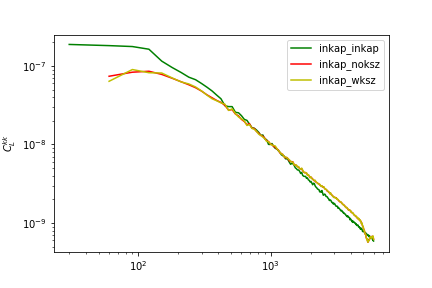
\includegraphics[width=0.8\textwidth]{cross_correlation3.png}
\caption{Auto-correlation of input lensing convergence, cross-correlation of input lensing convergence and reconstructed lensing convergence with reionization ksz, Cross-correlation of input lensing convergence and reconstructed lensing convergence without reionization ksz, }
\end{figure}

I am now simulating the bias and trying to understand the bias quantitatively. Since I am now fixing the bugs in this pipeline, the results shown below is not the conclusion. This work is also expected to be helpful for seperating reionization kSZ signals from lensing signals.



\bibliography{references}

\end{document}